\section{Análises Complementares}

\label{sec:analises-complementares}

As seções anteriores mostraram quanto esforço cada cenário exigiu, mas não explicaram por que os erros ocorreram nem o que foi feito para corrigi-los. Esta seção investiga esses pontos a partir da coluna Observações da execução final, na qual registramos, em texto livre, a mensagem de erro do Cypress de cada tentativa malsucedida e as alterações feitas para que o teste passasse. A análise é qualitativa por codificação \cite[Cap.~7.7.2, p.~99--101]{Wohlin2012}, e cada conclusão se apoia nos registros tentativa a tentativa, formando uma cadeia de evidências \cite[p.~99]{Wohlin2012}.

\subsection{O que foi alterado para o teste passar}
\label{subsec:correcoes}

Em todas as tentativas da execução final foram mantidos o mesmo modelo (GPT-4o), o mesmo \textit{system prompt} e a mesma aplicação. Dentro de um mesmo cenário, o que muda de uma tentativa para a seguinte é, portanto, o BDD ou o acaso do modelo. Para cada cenário que precisou de mais de uma tentativa, a alteração foi classificada a partir do registro dos autores na tentativa bem-sucedida. A classificação usou o texto das observações, e não a comparação automática da coluna do cenário BDD entre execuções, porque essa coluna nem sempre reflete as alterações descritas (por exemplo, na US36-CA00 e na US09-CA02). A Tabela~\ref{tab:correcoes} apresenta o resultado.

\begin{table}[htb]
\centering
\caption{Cenários que precisaram de correção e tipo de correção aplicada}
\label{tab:correcoes}
\begin{tabular}{lcl}
\hline
\textbf{Cenário} & \textbf{Execuções} & \textbf{Tipo de correção} \\
\hline
US06-CA00 & 6 & Aspas removidas do texto do passo \\
US09-CA02 & 4 & Seletor ou ID trocado \\
US04-CA00 & 3 & Seletor ou ID trocado \\
US05-CA00 & 3 & Índice [N] acrescentado \\
US16-CA00 & 3 & Sem alteração no BDD \\
US25-CA00 & 3 & Sem alteração no BDD\textsuperscript{*} \\
US40-CA00 & 3 & Índice [N] acrescentado \\
US41-CA00 & 3 & Passo removido ou BDD reformulado \\
US01-CA02 & 2 & Seletor ou ID trocado \\
US08-CA01 & 2 & Seletor ou ID trocado \\
US09-CA04 & 2 & Índice [N] acrescentado \\
US25-CA01 & 2 & Seletor ou ID trocado \\
US34-CA00 & 2 & Seletor ou ID trocado \\
US35-CA00 & 2 & Seletor ou ID trocado \\
US36-CA00 & 2 & Passo removido ou BDD reformulado \\
\hline
\end{tabular}
\legend{Fonte: Autores (2026).}
\end{table}

Dos 15 cenários que precisaram de correção, 13 (86,7\%) foram resolvidos alterando a escrita do BDD: troca do seletor ou do ID do elemento (7), inclusão do índice [N] para elemento repetido (3), remoção das aspas do texto do passo (1) e remoção de passo ou reformulação do BDD (2). Na US36-CA00, por exemplo, o passo que verificava o \textit{status} ``Arquivado'' teve de ser removido porque o texto nunca aparece naquele elemento. Na US41-CA00, o BDD foi reformulado com um novo ID para o menu Processos. Em apenas 2 cenários (13,3\%), US16-CA00 e US25-CA00, o teste passou na última tentativa sem nenhuma alteração no BDD em relação à anterior, o que sugere variabilidade do modelo. Na US25-CA00, porém, a primeira falha já havia exigido uma troca de seletor no BDD (Seção~\ref{subsec:imprevisibilidade}).

Como o \textit{system prompt}, o modelo e a aplicação não mudaram, podemos afirmar que esse padrão é compatível com a hipótese de que a forma de escrita do BDD influencia a qualidade do código gerado (Métrica 1.9).

\subsection{Causas das falhas}
\label{subsec:causas-erros}

Cada uma das 27 execuções com resultado N foi analisada individualmente a partir da mensagem real do Cypress registrada nas observações, de modo análogo à categorização de erros feita por \citeonline[p.~3224--3225]{Nettur2025} a partir do \textit{log} do Cypress. Cada mensagem recebeu um código de causa, resultando em oito categorias (Tabela~\ref{tab:categorias} e Figura~\ref{fig:classificacao-falhas}).

\begin{table}[htb]
\centering
\footnotesize
\caption{Classificação das 27 falhas por categoria de causa}
\label{tab:categorias}
\begin{tabular}{p{3.6cm}p{7.4cm}cc}
\hline
\textbf{Categoria} & \textbf{Descrição} & \textbf{Falhas} & \textbf{\%} \\
\hline
Seletor dinâmico instável & ID ou classe gerado automaticamente pelo \textit{framework} de interface (React, Chakra, Emotion) não corresponde ao DOM real & 9 & 33,3\% \\
Seletor genérico ou ambíguo & O seletor casa com vários elementos da tela e o Cypress rejeita o clique & 6 & 22,2\% \\
Erro de geração de código & Texto do passo diverge entre o arquivo \texttt{.feature} e a \textit{step definition}, ou há definições duplicadas & 6 & 22,2\% \\
Elemento repetido sem indexação & Elemento duplicado na tela, sem [N] ou \texttt{.eq(N)} para desambiguar & 2 & 7,4\% \\
BDD descreve comportamento incorreto & O texto ou a condição esperada nunca ocorre na aplicação & 1 & 3,7\% \\
Erro de digitação no texto gerado & Um erro de digitação alterou a \textit{string} esperada na asserção & 1 & 3,7\% \\
Lógica de asserção de texto & A asserção esperava uma \textit{string} concatenada, mas o DOM tem parágrafos separados & 1 & 3,7\% \\
Variabilidade pura do modelo & Com o BDD idêntico, a nova tentativa interpretou corretamente sozinha & 1 & 3,7\% \\
\hline
\end{tabular}
\legend{Fonte: Autores (2026).}
\end{table}

\begin{figure}[htb]
\centering
\caption{Classificação das 27 falhas por categoria de causa}
\label{fig:classificacao-falhas}
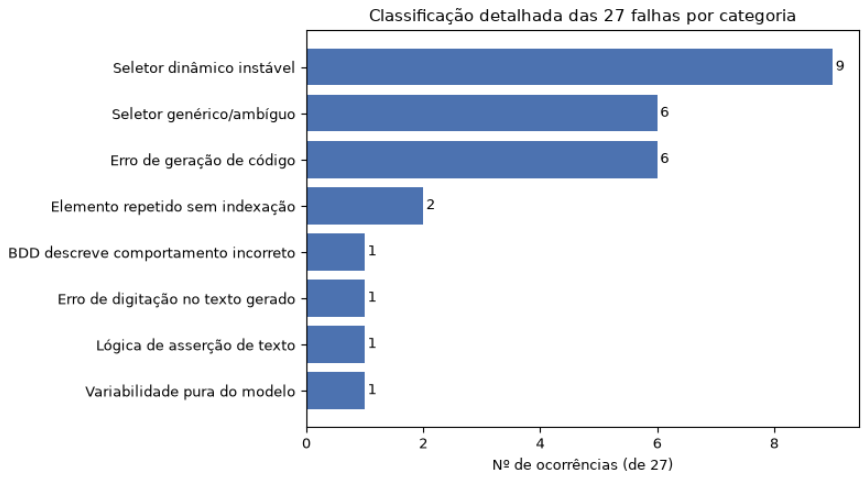
\includegraphics[width=0.9\textwidth]{figuras/classificacao_erros.png}
\legend{Fonte: Autores (2026).}
\end{figure}

Apoiando-se na estruturação hierárquica de códigos descrita por \citeonline[p.~100]{Wohlin2012}, as oito categorias foram agrupadas em quatro grupos de causa raiz (Tabela~\ref{tab:grupos} e Figura~\ref{fig:indicador-final}).

\begin{table}[htb]
\centering
\footnotesize
\caption{Causa raiz das 27 falhas, agrupada em quatro grupos}
\label{tab:grupos}
\begin{tabular}{p{4.4cm}p{6.6cm}cc}
\hline
\textbf{Grupo de causa raiz} & \textbf{Categorias reunidas} & \textbf{Falhas} & \textbf{\%} \\
\hline
Relacionado ao elemento de interface & Seletor dinâmico instável, seletor genérico ou ambíguo, elemento repetido sem indexação & 17 & 63,0\% \\
Erro de geração de código & Erro de geração de código & 6 & 22,2\% \\
BDD ou asserção não corresponde ao comportamento real da aplicação & BDD descreve comportamento incorreto, erro de digitação, lógica de asserção de texto & 3 & 11,1\% \\
Variabilidade pura do modelo & Variabilidade pura do modelo & 1 & 3,7\% \\
\hline
\end{tabular}
\legend{Fonte: Autores (2026)}
\end{table}

\begin{figure}[htb]
\centering
\caption{Causa raiz das 27 falhas, agrupada em quatro grupos (\% das falhas)}
\label{fig:indicador-final}
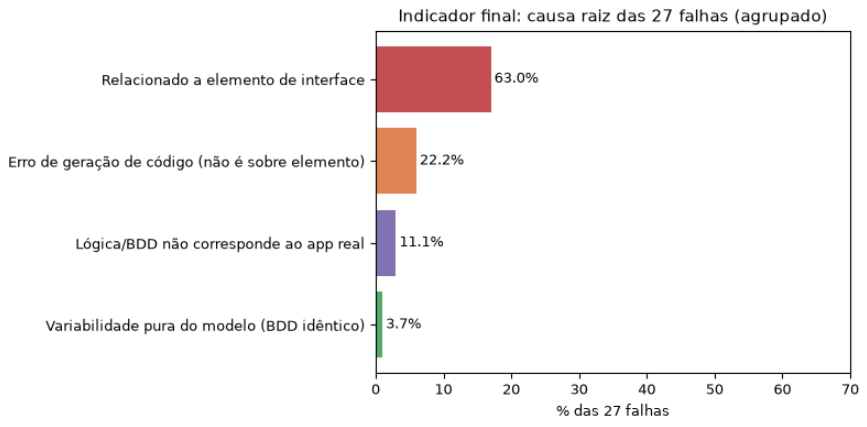
\includegraphics[width=0.85\textwidth]{figuras/causa_raiz.png}
\legend{Fonte: Autores (2026).}
\end{figure}

A maior parte das falhas, 63,0\% (17 de 27), está diretamente relacionada a como o elemento de interface foi referenciado no BDD. Os seletores dinâmicos instáveis, como o \texttt{\#tabs-:r17:--tab-5} da US25-CA00, são gerados pelo \textit{framework} a cada renderização e deixam de corresponder ao elemento real. Os seletores genéricos casam com vários elementos, como na US41-CA00, em que o ID usado para o menu Processos aparecia sete vezes na tela. Já os elementos repetidos ficaram sem o índice [N] que os diferenciariam. Em todos esses casos, a origem do erro está na própria referência ao elemento escrita no BDD.

O interessante é que o CAPJu não foi desenvolvido pensando em testes automatizados, considerando que percebemos a falta de IDs estáveis em elementos importantes da interface. Isso foi contornado com seletores CSS, que funcionam como um endereço para um ponto específico da página quando não há ID disponível. Os resultados podem, por isso, ser mais pronunciados do que em aplicações preparadas para automação.

Os 37,0\% restantes têm origem mista (geração de código pela IA, notação do BDD, conteúdo do BDD ou variabilidade do modelo) e não foram atribuídos individualmente à escrita do BDD. Há ainda uma incerteza sobre o grupo de 11,1\%: na US16-CA00, as falhas por erro de digitação e por lógica de asserção desapareceram sem nenhuma alteração no BDD (Seção~\ref{subsec:correcoes}), o que sugere que parte delas também decorre da variabilidade do modelo. Os percentuais referem-se às 27 tentativas com falha, e não aos 15 cenários corrigidos da Seção~\ref{subsec:correcoes}.

\subsection{Imprevisibilidade da IA: dois casos}
\label{subsec:imprevisibilidade}

Dois cenários ilustram a imprevisibilidade do modelo mesmo com um \textit{system prompt} robusto: um erro de geração sensível à notação do BDD (US06-CA00) e um caso em que o mesmo BDD produziu resultados diferentes (US25-CA00). A Tabela~\ref{tab:casos} reúne a evidência registrada tentativa a tentativa.

\begin{table}[htb]
\centering
\footnotesize
\caption{Sequência de tentativas dos cenários US06-CA00 e US25-CA00}
\label{tab:casos}
\begin{tabular}{p{1.6cm}p{1.25cm}p{1.35cm}p{4.8cm}p{4.4cm}}
\hline
\textbf{Cenário} & \textbf{Tent.} & \textbf{Result.} & \textbf{Erro registrado} & \textbf{Alteração no BDD antes da tentativa seguinte} \\
\hline
US06-CA00 & 1 & N & \textit{Step implementation missing} (divergência de aspas entre o arquivo de \textit{feature} e a \textit{step definition}) & Nenhuma no texto dos passos \\
US06-CA00 & 2 a 5 & N & \textit{Multiple matching step definitions} (duas definições com a mesma assinatura) & Nenhuma no texto dos passos até a 5ª (na 4ª, só o seletor entre parênteses foi reescrito, sem efeito); após a 5ª, aspas duplas removidas do texto do BDD \\
US06-CA00 & 6 & S & -- & -- \\
\hline
US25-CA00 & 1 & N & ID dinâmico \texttt{\#tabs-:r17:--tab-5} não encontrado & Seletor trocado por \texttt{button[role="tab"]} \texttt{[data-index="5"]} \\
US25-CA00 & 2 & N & A asserção não considerou as colunas Ações, Servidor, Diretor e Administrador como quatro verificações distintas & Nenhuma \\
US25-CA00 & 3 & S & -- & -- \\
\hline
\end{tabular}
\legend{Fonte: Autores (2026).}
\end{table}

Na US06-CA00, o texto dos passos não mudou nas cinco primeiras tentativas, e os erros foram de geração de código: primeiro uma divergência de aspas e depois, repetidamente, definições duplicadas. Só na sexta tentativa o teste passou, depois que as aspas duplas foram removidas do BDD. Isso sugere que uma pequena alteração de notação pode produzir erros repetidos mesmo com um \textit{system prompt} mais técnico.

Na US25-CA00, a primeira falha decorreu de um seletor dinâmico, corrigido no BDD. A segunda ocorreu porque o modelo não interpretou que o passo das quatro colunas descrevia quatro verificações separadas. Na terceira tentativa, com o BDD idêntico ao da segunda, o teste passou, e o modelo passou a interpretar corretamente a mesma instrução. Esse caso evidencia a natureza de caixa-preta do modelo e sua variabilidade, onde com o BDD e \textit{system prompt} fixos, o resultado pode variar entre execuções. Esse achado sustenta a limitação de que não há garantia de sucesso na primeira execução.
